% Zeitbereich & Bildbereich Darstellung
% Flussdiagramm?

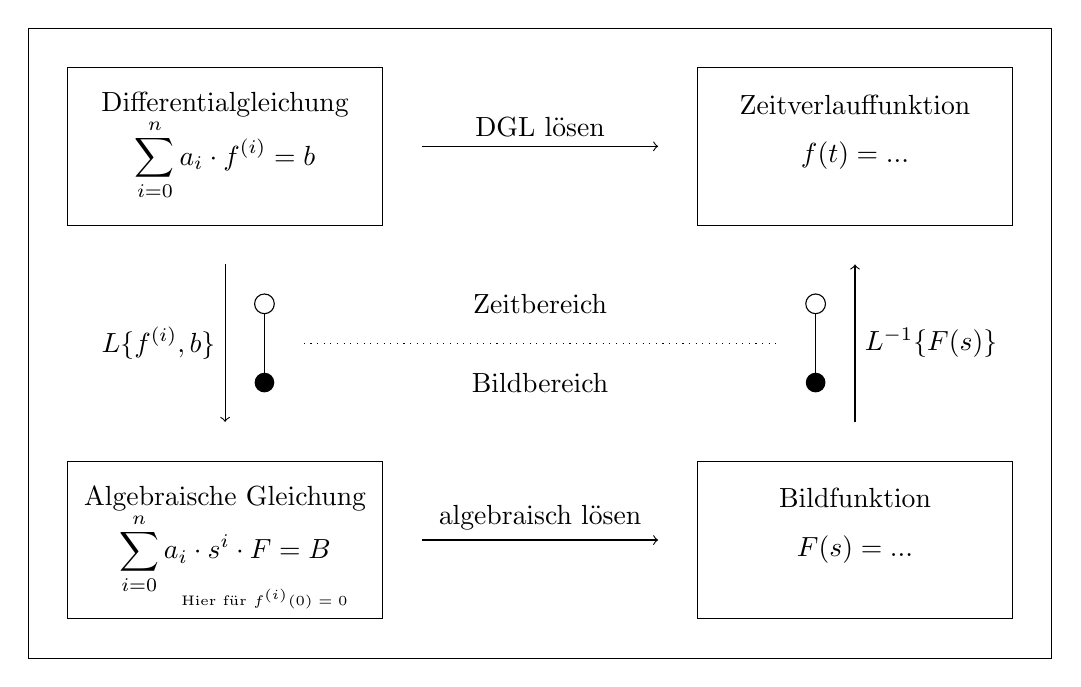
\begin{tikzpicture}
    \draw (-0.5,2.5) rectangle (12.5,-5.5);
    % Zeitbereich
    \draw (0,0) rectangle (4,2);
    \draw (6,1.5) node[align=center]{};
    \draw[->](4.5,1) -- (7.5,1) node[pos=0.5, above]{DGL lösen};
    \draw (8,0) rectangle (12,2);
    % Text Zeitbereich 1.Kasten
    \draw (2,1) node[align=center,text centered]{Differentialgleichung\\%
    $\displaystyle{
        \sum_{i=0}^{n} a_i \cdot f^{(i)}  = b} 
    $};

    % Text Zeitbereich 2.Kasten
    \draw (10,1) node[align=center, text centered]{Zeitverlauffunktion\\$\displaystyle{f(t)=... \vphantom{\sum_{i=0}^{n}}}$};
    
    % Laplace Transformationszeichen + Pfeil
    \draw(2.5,-1) circle (0.125);
    \draw(2.5,-1.125) -- (2.5,-1.875);
    \fill[black](2.5,-2) circle (0.125);
    \draw [->](2,-0.5) --(2,-2.5) node[pos=0.5, left]{$\mathscr{L}\{f^{(i)},b\}$};

    % Bildbereich
    \draw (0,-5) rectangle(4,-3);

    \draw[->](4.5,-4) -- (7.5,-4) node[pos=0.5, above]{algebraisch lösen};
    \draw (8,-5) rectangle(12,-3);

    % Text Laplacebereich 1.Kasten
    %\draw (2,-2.75) node[align=center,text centered]{\tiny Anm.: Nur wenn $f^{(i)}(0) = 0$, so gilt:};
    %\draw (2,-4.75) node[align=center,text centered]{\tiny Spezialfall!};
    \draw (2.5,-4.75) node[align=center,text centered]{\tiny Hier für $f^{(i)}(0) = 0$};
    \draw (2,-4) node[align=center,text centered]{Algebraische Gleichung\\%
    $\displaystyle{
        \sum_{i=0}^{n}a_i \cdot 
        \smash{
            %\underbrace{
                s^{i} \cdot F
            %}_{
            %    \rlap{\tiny wenn $\mathrlap{f^{(i)}(0) = 0}$}
            %}
        } = B \vphantom{\sum{i=0}^{n}}}%
    $};

    % Text Laplacebereich 2.Kasten
    \draw (10,-4) node[align=center, text centered]{Bildfunktion\\$\displaystyle{F(s)=... \vphantom{\sum_{i=0}^{n}}}$};
    

    % Laplace Transformationszeichen + Pfeil
    \draw(9.5,-1) circle (0.125);
    \draw(9.5,-1.125) -- (9.5,-1.875);
    \fill[black](9.5,-2) circle (0.125);
    \draw[->](10,-2.5) -- (10,-0.5) node[pos=0.5, right]{$\mathscr{L}^{-1}\{F(s)\}$};

    % Trennung Zeit- und Bildbereich
    \draw(6,-1) node [align=center] {Zeitbereich};
    \draw[dotted](3,-1.5)--(9,-1.5);
    \draw(6,-2) node [align=center] {Bildbereich};

\end{tikzpicture}
